% \clearpage
\subsection{Tópicos de pesquisa a serem investigados}
\label{ch:proposal}
%As Visões atuais da 
No futuro da Internet, a maior parte do fluxo do tráfego da rede será provido por nós na borda~\cite{cisco:forecast2017}.
Dentro desse contexto, 
%as arquiteturas de rede 5G devem prover um ambiente de comunicação capaz de superar as deficiências de infraestrutura das redes atuais. 
As redes se tornarão muito mais densas dado a diversidade de células instaladas com tamanho cada vez menor, bem como uma comunicação direta de dispositivo-para-dispositivo. As células pequenas, como BS e Femto BS,
são capazes %de melhorar a cobertura e a capacidade da rede em relação as células maiores, e elas serão capazes de transportar a maior parte do trafego.
de diminuir a sobrecarga de retorno do tráfego e ajuda prover baixa latência aos serviços de vídeo streaming~\cite{guan:2019:CLC}.

A Figura~\ref{fig:scenario-ex-lte-wifi} exemplifica um cenário interessante a ser estudado, uma rede multinível heterogênea com uma célula macro e algumas células metro e pico são usadas para retransmissão. Através dessas pequenas células internas e externas de baixo custo o usuário pode ser capaz implementar ambientes domésticos e privados internos com baixo custo.

\vspace{0.8cm}
\begin{figure*}[htpb]
	\centering
	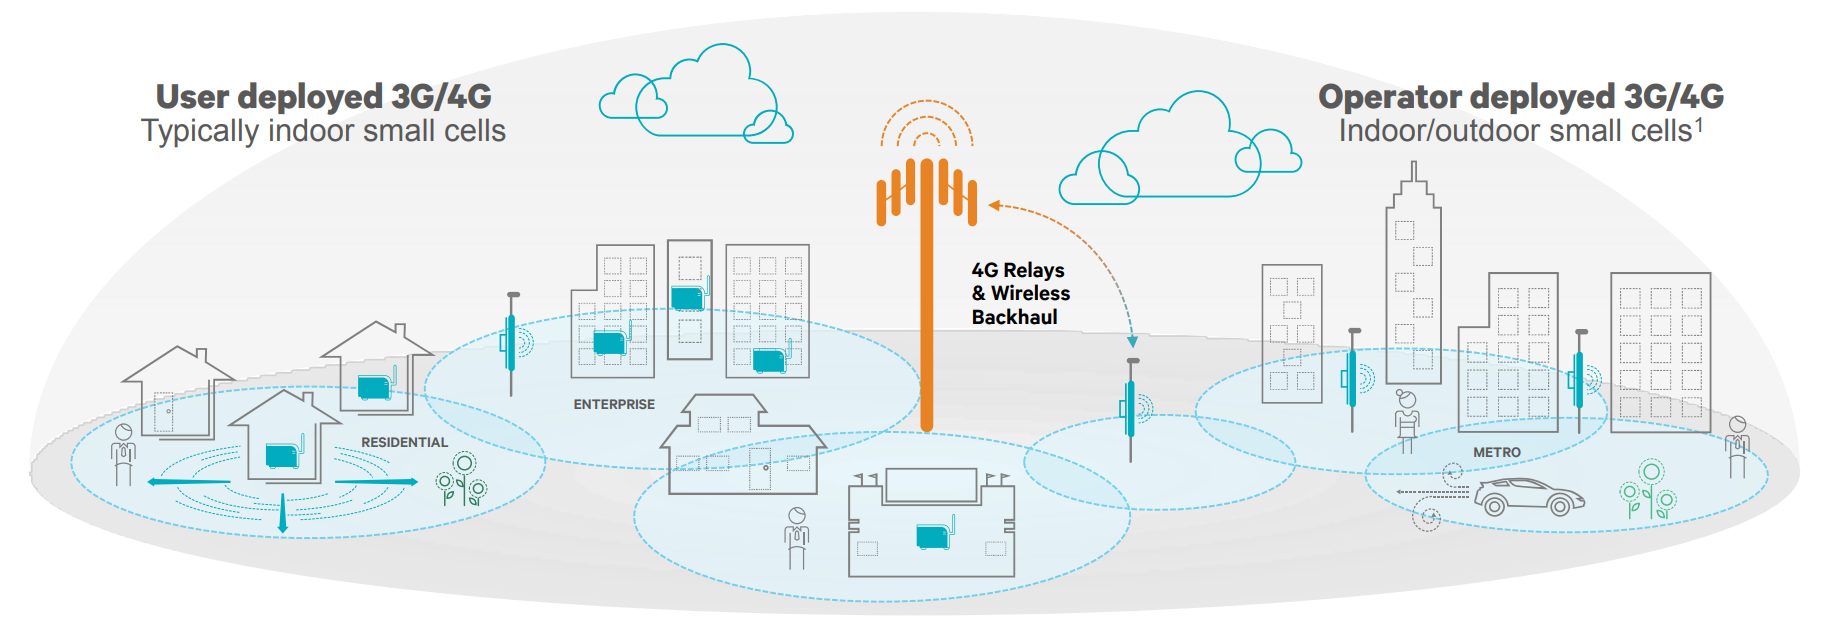
\includegraphics[width=0.85\textwidth]{img/hetnet-lte-wifi-v2.png}
% 	\vspace{-1cm}
	\caption{Exemplo de cenário de redes multinível heterogêneas~\cite{Qualcomm2013}.}
	\label{fig:scenario-ex-lte-wifi}
\end{figure*}
%\vspace{0.8cm}

As subseções seguintes apresentam algumas ideias principais para a continuidade deste projeto de pesquisa baseado no cenário acima. Os tópicos de pesquisa a serem abordados estão divididos em três tópicos, que são
detalhado em Seções seguintes. Cada tópico abrange a motivação e objetivos.

%=============================================================================%
%\subsection{Topicos de pesquisa}
%\label{sec:topics}

%Devido ao compartilhamento de ambientes de rede, a natureza do \textit{best-effort} da infraestrutura da Internet, e o comportamento egoísta totalmente isolado dos jogadores da HAS discutidos na seção 3. É difícil para streams de vídeo satisfazer os três objetivos descritos abaixo. Desde de que existam multiplos clientes concorrentemente competindo entre eles um limitado comprimento de onda, as soluções existentes para clientes dirigido a HAS não trabalham vem e sofrem muitos problemas com perda de pacotes, flutação de comprimento de onda, oscilações na qualidado e troca de taxas de bits~(Instabiliddade do vídeo mostrada ba Figura~\TODO{Falta gerar gráfico}), QoE indesejavel e compartilhamento de recursos da rede, recursos da rede inutilizados ou sobrescritos do qual 'will adversely affect the viewer's QoE'.% Alem disso, estes problemas tem sido confirmados em experimentos recentas. 

%Os tópicos de pesquisa a serem abordados estão divididos em três tópicos, que são
%detalhado em Seções seguintes.
%Cada tópico abrange a motivação e os objetivos.

%-----------------------------------------------------------------------------%
\subsubsection{Mecanismos Cooperativos para Streaming de Video}
\label{subsec:video-streaming}

Dentro do ambiente de rede multinível compartilhado, em que muitos reprodutores DASH competem pela largura de banda disponível, várias flutuações repentinas na banda da rede podem ocorrer ao longo do tempo.
% 
A seção~\ref{subsec:evaluation} mostra a influência que os mecanismos ABR têm na variação de escolhas da taxa de bits do próximo segmento, onde o QoE do usuário estava diretamente relacionado ao processo de decisão que ele utiliza. Além disso, o trabalho~\cite{bentaleb:2018:MSys} também mostra algumas armadilhas que podem ocorrer devido ao comportamento totalmente isolado dos clientes HAS~(ou seja, essas soluções estão funcionando independentemente, sem coordenação). Em particular, a presença de vários clientes HAS simultâneos que competem pelos recursos de rede compartilhados podem causar problemas de escalabilidade do HAS, incluindo (i) instabilidade de video devido à troca de taxa de bits frequente, no qual os usuários competem por um link de gargalo em um ambiente de rede compartilhado e oscilações de qualidade perceptual; (ii) injustiça de QoE; e (iii) subutilização ou subscrição excessiva de recursos de rede. Esses problemas são agravados quando o número de usuários aumenta e no caso de ambientes heterogêneos. Esses problemas continuam sendo uma preocupação séria para os operadores de rede e provedores de conteúdo. 
Neste contexto, é desejavel ter mecanismos computacionais que identifiquem automaticamente o processo de decisão do HAS de cada video antes de escalona-los.
\emph{Os objetivos para este tópico de pesquisa são:}

\begin{itemize}
%  	\itemsep0pt
    \item Realizar um estudo detalhado sobre os processos de decisão cooperativos existentes;
    \item Propor mecanismos cooperativos entre grupos de usuários para auxiliar no processo de decisão do algoritmo ABR. Além disso, esses mecanismos podem facilitar a cooperação de \textit{download} e \textit{upload} de um mesmo conteúdo entre os usuários de uma mesma rede; 
    \item Implementar e avaliar as soluções propostas utilizando ambientes controlados.
\end{itemize}

% \textit{O objetivo neste tópico de pesquisa} é implementar mecanismos cooperativos capazes de identificar eficientemente o processo de decisão de cada cliente. Além disso, esses mecanismos podem facilitar a cooperação de download e upload de um mesmo conteúdo entre os usuários de uma mesma rede. Para isso, será implementado mecanismos que auxiliem o reprodutor podendo-se utilizar de Teoria dos Jogos~(GT) nesta tarefa, composto por três estágios principais: entrada, processamento e saída. Os requisitos de QoE do video podem ser as entradas do sistema. Essas entradas serão mapeadas para as funções apropriadas de associação e valores de verdade.

% As abordagens mencionadas em \autoref{subsec:arch-cloud-fog} podem diminuir a carga de tráfego 
% e melhorar a QoE. No entanto, também existem armadilhas devido ao comportamento egoísta totalmente isolado (ou seja, essas soluções estão funcionando independentemente, sem coordenação) dos players do HAS, seus esquemas HAS possuem os seguintes quatro grandes problemas:
% \begin{itemize}
%     \item Multi-player Problemas: Por padrão, o design do reprodutor de video se esforça individualmente para buscar os segmentos de video com a maior taxa de bits
% \end{itemize}



%-----------------------------------------------------------------------------%
\subsubsection{Arquitetura de Distribuição de Video Multinível}
\label{subsec:sca-contrl-arch}

%Com a melhoria de largura de banda que foi feita nos links de acesso e nas redes de backbone, os usuários finais agora esperam que aplicativos de vídeo de alta qualidade funcionem em qualquer lugar e em uma variedade de dispositivos heterogêneos. Recentemente, como uma das novas arquiteturas de rede evolutiva, a Rede Centrada na Informação~(ICN)~[337] foi proposta para facilitar aplicativos como disseminação de conteúdo e serviços de streaming de alta qualidade (por exemplo, aplicativos de streaming de vídeo multicast baseados em HAS, etc.). No entanto, vários desafios, incluindo a cooperação com o cache na rede, o encaminhamento de múltiplos caminhos e o controle de qualidade ou congestionamento, ainda precisam ser enfrentados antes da implantação do serviço na Internet. De fato, a maioria dos trabalhos relacionados é baseado em várias suposições nas quais, por exemplo, aplicativos de destino são apenas aplicativos não em tempo real, a rede de destino deve ser uma pequena rede de gerenciamento ou uma rede com fio~(ou sem fio) e assim por diante. 
%
%Paralelamente, 
%Os recursos de borda dos ISPs ou usuários finais podem ser utilizados para hospedar o conteúdo de vídeo na proximidade dos usuários finais, reduzindo a latência e mitigando a carga nas redes principais e nos data centers. Isso será útil para o cenário de transmissão ao vivo que requer uma latência baixa. 
%
%
%Além disso, a integração de serviços baseados em HAS em tais mecanismos de comunicação requer uma avaliação rigorosa em bancos de testes realistas antes da implantação. O principal objetivo é analisar e investigar a integração da entrega de vídeo baseada em HAS nas redes futuras, onde:
%
%%***********Objectives of the proposal***********
%1. How to deliver high quality streaming using in-Network coding and caching?
%2. How to enable the multipath and multicast capabilities for HAS in future networks like ICN?
%3. What is the impact of these networks on HAS decisions?
%4. What is the benefits that edge computing can add in HAS over the future networks?
%5. What is the deployment cost?

Um ambiente multinível pode ser composto por mais de um domínio de dispositivos. Por sua vez, 
os recursos de cada domínio podem ser utilizados para hospedar o conteúdo de vídeo na proximidade dos usuários finais, reduzindo a latência e mitigando a carga nas redes principais da nuvem.
Para integrar os serviços DASH em tais ambientes de comunicação, o nó névoa requer a implantação de entidades extras para realizar a transmissão do vídeo.
Dentro desse contexto, 
mecanismos para realizar a integração entre esquemas ABR e o streaming do vídeo podem melhorar o QoE em cada nível da rede, \emph{os objetivos para este tópico de pesquisa são:}  

% algumas características em tais ambiente multiníveis precisam ser mais estudados, como alocação de cache, posicionamento, tomadas de decisões em tempo real. 

% além do que pode ser alcançado por ABR e cache executando individualmente

% Por exemplo, um cache dentro de um dispositivo capaz de provisionar um conjunto de diferentes partes de conteúdo pode apresentar diferentes nível de granularidade. Logo um nível diferente de granularidade surge em tais dispositivos de ponto de acesso. Se a granularidade de certas áreas se tornar muito fina, novos problemas de escalabilidade começam a aparecer. Dividir o conteúdo entre os nós da névoa no nível certo de granularidade é um problema complexo por si só. % Assumindo cenários federados com domínios diferentes na névoa é necessária.

% Additionally, orchestrator could combine both  ABR  and  cache  schemes  in  each  tier  to  improve  the  QoE,  beyond  that  which  can  be achieved by either ABR and caching running individually.   The orchestrator must also deal with  users  mobility  between  different  locations  quite  often  in  the  current  wireless  network scenarios, which hamper the delivery of videos with QoE support. 

%Um cenário simples é que um shopping center pode implantar muitos nós de névoa em diferentes andares para fornecer Acesso Wi-Fi e entregar alguns serviços envolvidos (ou seja, navegação interior, distribuição de anúncios, coleções de feedback) para seus clientes. No entanto, no tempo de pico, as capacidades desses nós de nevoeiro não podem servir eficientemente os clientes. Enquanto isso, o provedor de névoa, aqui é o centro comercial, pode estender sua infraestrutura, pagando os recursos de computação e armazenamento terceirizados dos nós de nuvem, que pode ser máquina virtual (VM) alugada de provedores de nuvem em uma base de pay-per-use. Todos os nós de processamento distribuídos (nuvem ou névoa) são gerenciados por um corretor de recursos, que é um componente de gerenciamento de recursos e um planejador para os fluxos de trabalho enviados pelos usuários no lado do nevoa. 
%Neste caso, uma agenda de tarefas, que pode minimizar o tempo de conclusão do fluxo de trabalho, mas corresponde a uma grande quantidade de custo monetário, não é uma solução ideal para fornecedores da fog. 
%Assim, neste artigo, propomos um algoritmo de escalonamento de tarefas que pode conseguir uma boa compensação entre o tempo de execução do fluxo de trabalho e o custo pelo uso dos recursos da nuvem. Os resultados experimentais mostram o excelente desempenho do nosso método comparado com alguns outros trabalhos.	

%Com novas possibilidades sendo criadas para oferecer melhores serviços e o funcionamento da internet. Enquanto a rede se torna mais robusta, o problema se torna mais complexo e surgem novos desafios. Para adaptar um sistema CDN com ambiente de várias camadas ao nevoeiro, diferentes características devem ser estudadas, como alocação de cache, posicionamento, substituição e seleção, geralmente, tomada de decisões em tempo real. Como diferentes tamanhos de cache, sendo alocados nas camadas para armazenar um intervalo de conteúdo para provisionar uma região. Além disso, um tamanho de cache em um dispositivo AP deve ser capaz de lidar com um conjunto de diferentes partes de conteúdo, para que os usuários finais possam ter garanias de QoE. Assim, surge um nível diferente de granularidade nos dispositivos de ponto de acesso. Se a granularidade de certas áreas se tornar muito granularidade, problemas de escalabilidade começam a aparecer. Dividir o conteúdo do nevoeiro na rede pelos APs no nível certo de granularidade é um problema complexo por si só.

\begin{itemize}
%  	\itemsep0pt
	\item Realizar um estudo sobre a arquitetura DASH em tais ambiente multiníveis assumindo cenários com diferentes domínios;

    \item Verificar as aproximações atuais na literatura para implantação desse tipo de serviço, analisar qual o trade-off entre o custo para as operadoras e aprimoramento do QoE;
    
    \item Propor mecanismos para melhorar esse esse processos de decisão de provisionamento do conteúdo;
    
    \item Implementar e avaliar a solução proposta em ambientes controlados.%, para isso o uso do simulador integrado a biblioteca libdash pode ser utilizados.   
\end{itemize}


%No entanto, é preciso projetar algumas extensões para permitir o streaming de video a um grande número de usuários heterogeneos. 
%
%No entanto, como são basicamente projetados para funcionar com as redes IP ponto a ponto tradicionais, geralmente limitadas a um único sistema autônomo, elas requerem algumas extensões para permitir o streaming de vídeo de alta qualidade a um grande número de usuários heterogêneos na ampla Internet. 
%
%A tendência para a computação de borda e neblina deve ser integrar às abordagens de gerenciamento de tráfego de vídeo
%
%A tendencia entre esses diferentes dominios - diferentes dispositivos podem compor um dominio da névoa. . Os recursos de borda dos ISPs ou usuários finais podem ser utilizados para hospedar o conteúdo de vídeo na proximidade dos usuários finais, reduzindo a latência e mitigando a carga nas redes principais e nos data centers. Isso será útil para o cenário de transmissão ao vivo que requer uma latência baixa. Além disso, a integração de serviços baseados em HAS em tais mecanismos de comunicação requer mais analises e investigar a integração da entrega de vídeo baseada em HAS nas redes futuras
%
%Os paradigmas SDN/NFV são tecnologias notáveis para controlar não apenas os fluxos de comunicação, mas também as funções de serviço nas redes. 
%Além disso, a tendência para a computação de borda e neblina deve ser integrada às 
%
%Para integrar uma arquitetura de Multinivel Névoa/Nuvem às abordagens de gerenciamento de tráfego de vídeo, este trabalho tem como objetivo abordar algumas das seguintes questões de pesquisa:~\textit{i)} Como determinar as melhores camadas para alocação de serviços de vídeo?~\textit{ii)} Como os pedaços de vídeo não solicitados devem ser distribuídos na hierarquia de borda/nuvem, considerando as informações de localização do usuário e estimativas sobre a localização futura do usuário em tempo real?~\textit{iii)} Como facilitar o streaming de vídeo através de várias fontes simultaneamente?~\textit{iv)} Como os algoritmos ABR são afetados pela arquitetura proposta?
%
%Dada a arquitetura do modelo de serviço e ambiente de nuvem/borda de várias camadas,. Este ambiente Névoa/Nuvem pode ser composto por um mais dominios na Névoa.
%
% este trabalho tem como objetivo abordar algumas das seguintes questões de pesquisa:~\textit{i)} Como determinar as melhores camadas para alocação de serviços de vídeo?~\textit{ii)} Como os pedaços de vídeo não solicitados devem ser distribuídos na hierarquia de borda/nuvem, considerando as informações de localização do usuário e estimativas sobre a localização futura do usuário em tempo real?~\textit{iii)} Como facilitar o streaming de vídeo através de várias fontes simultaneamente?~\textit{iv)} Como os algoritmos de adaptação à taxa de bits podem ser afetados pelo tamanho do pedaço de vídeo em uma arquitetura de várias camadas?
%
%Parta lidar com a escalabilidade necessária em ambientes de cidades inteligentes.
%% Este projeto tem como objetivo considerar ambientes multiníveis que utilizem tecnologia emergentes~(4G, 5G, WiFi) para a entrega do vídeo. Para COm isso, novos desafios surgem nesse processo integração. 
%projetar uma entrega de vídeo com diferentes dominios mantendo garantias de QoE em ambientes de cidades inteligentes~\cite{gamaUCC2019, KreuzbergerWorkshop2016}. O esquema proposto aproveitará de tecnologias emegerntes relacionadas à redes~(como 5G e WiFi).% A Figura~\ref{fig:scenario-arch} descreve, no lado esquerdo, uma arquitetura de rede de várias camadas, composta por um conjunto heterogêneo de dispositivos e aplicativos que utilizam recursos de computação distribuídos por meio de uma tecnologia de comunicação de acesso múltiplo, como 5G e WiFi. Este projeto propõe estender o streaming de vídeo DASH para suportar conectividade simultânea de caminhos múltiplos~\cite{poliakovPHD2018, Velasquez2018}.
%\emph{O objetivo neste tópico de pesquisa} é realizar um estudo sobre a arquitetura DASH disponíveis com diferentes dominios. 
%Assumindo cenários em que a federação entre diferentes provedores de serviços da névoa é necessária.
%
%\begin{itemize}
%    \item Analisar atuais aproximações na literatura para implantação desse tipo de serviço, qual o trade-off entre o custo para as operadoras e aprimoramento do QoE.
%    \item propor mecanismos a nível de provedor de conteúdo para melhorar esse esse processos de decisão estudados.
%    \item Implementar e avaliar a solução proposta em ambientes controlados, para isso o uso do simulador ns-3 integrado a biblioteca libdash podem ser utilizados.   
%\end{itemize}
%O lado direito da Figura~\ref{fig:scenario-arch} descreve parte dos parâmetros que devem ser avaliados para definir quais serviços de vídeo precisam ser implantados, juntamente com a camada mais adequada para implantar cada um deles. Observe que os parâmetros na camada mais inferior para feedback diferem dos de outras camadas. Inicialmente, os parâmetros avaliados considerados incluem o perfil do usuário, a carga da célula local, a qualidade do link, a complexidade do movimento dos vídeos e também detalhes inteligentes da cidade, como a localização e a rota rastreada no caso de usuários com mobilidade. Alguns dos nós podem ser estacionários, mas outros podem variar de padrões de baixa a alta mobilidade, que podem ser levados em consideração para melhorar a qualidade da entrega de vídeo.

%-----------------------------------------------------------------------------%
\subsubsection{Redes heterogêneas em larga escala}
\label{subsec:mobility}

Com a diversidade de dispositivos, tipos de comunicação de rede e tipos de conteúdo. Em redes heterogêneas, a maioria dos usuário possuem mais de uma interface de rede~(e.g., 5G e WiFi) por onde o conteúdo multimídia pode chegar. Atualmente, poucos trabalhos em DASH abordam mecanismos apropriados para realizar a escolha dos tipos de comunicação com seus requisitos específicos.
É importante notar que haverá heterogeneidade na rede e diferentes requisitos de QoE, por exemplo, um smartphone tem um requisito de satisfação menor do que uma Smart TV, bem como os conteúdos de vídeo tem diferentes requisitos.

%Com novas possibilidades sendo criadas para oferecer melhores serviços bem como o funcionamento da internet. Enquanto a rede se torna mais robusta, o problema se torna mais complexo e surgem novos desafios. 

Outra questão interessante em redes de larga escala é como o tráfego cruzado (por exemplo, troca de arquivos) afeta a estimativa de largura de banda disponível. Em redes de larga escala o compartilhamento de recursos com diferentes tipos de tráfego dinâmicos causam uma flutuação na banda impactando as tomadas de decisão de algoritmos ABR.
%o impacto de configurações realistas em ambientes de Cidades Inteligentes nas tomadas de decisões feitas pelo algoritmos ABR.
Consequentemente, é necessária uma cooperação e coordenação eficiente entre os dispositivos e mecanismos efetivos de alocação e gerenciamento de recursos da rede para suprir a demanda dos atores do HAS, sua concorrência e a capacidade limitada da rede.



% Esperamos que uma pergunta natural seja como suporte à implantação em larga escala? Como se comportaria em uma rede heterogênea de área ampla, quando milhares de jogadores do HAS são implantados e competem? Nossa solução geralmente é projetada para ter um bom desempenho em um cenário de grande escala

% Nossas soluções podem combinar esquemas de ABR e cache em cada camada para melhorar a QoE, além do que pode ser alcançado pelo ABR e pelo cache executando individualmente.

\emph{Os objetivos para este tópico de pesquisa são: }  

\begin{itemize}
    % \item Investigando como oferecer suporte à implantação em larga escala e abordar a sobrecarga de comunicação e a heterogeneidade do sistema em sistemas de entrega HAS habilitados para SDN;
    % \itemsep0pt
    \item Investigar como dar suporte a implantação em larga escala e abordar a sobrecarga da rede;
    
    \item Modelar redes heterogêneas em larga escala para distribuição de video levando em consideração ambientes em Cidades Inteligentes;
    
    \item Inserir trafego cruzado para analisar o comportamento das soluções propostas em ambientes 
    estudados.
    %heterogêneos de larga escala.
\end{itemize}


%-----------------------------------------------------------------------------%
% \subsection{Gerenciamento de mobilidade distribuída}
% \label{subsec:mobility}

% O gerenciamento de mobilidade refere-se a um conjunto de mecanismos para manter a continuidade das sessões em andamento, enquanto que um usuário móvel altera seu ponto de acesso à rede.
% Na arquitetura DASH, o manifesto criado pelo servidor pode auxiliar em possíveis soluções no gerenciamento de mobilidade, além de realizar um preprocessamento com informação de controle relacionado à mobilidade e dados dos servidores. 
% %De acordo com~\citet{Valtulina2014}, essa abordagem centralizada torna o gerenciamento de mobilidade propenso a várias limitações de desempenho, como roteamento abaixo do ideal, baixa escalabilidade, potencial ponto único de falha e falta de granularidade para o serviço de gerenciamento de mobilidade.
% \emph{Os objetivos deste tópico de pesquisa são:}
% %item Inicialmente, os parâmetros avaliados considerados incluem o perfil do usuário, a carga da célula local, a qualidade do link, a complexidade do movimento dos vídeos e também detalhes inteligentes da cidade, como a localização e a rota rastreada no caso de usuários com mobilidade. Alguns dos nós podem ser estacionários, mas outros podem variar de padrões de baixa a alta mobilidade, que podem ser levados em consideração para melhorar a qualidade da entrega de vídeo.

% \begin{itemize}
% \item Realizar um estudo detalhado em soluções disponíveis para balanceamento de carga em redes móveis, que podem ser usadas para acionar procedimentos de transferência na arquitetura multinível;

% \item Examinar e propor mecanismos que devemos utilizar para lidar com a mobilidade do usuário.
% Como dividir o conteúdo e recursos computacionais;

% \item Analisar os mecanismos desenvolvidos para transferência em redes multiníveis, considerando a transferência sessões entre diferentes domínios.

% %\item Antes de alocar o serviço de streaming de video em DASH, quais serviços é necessário acrescentar para o provisionamento do conteúdo
% \end{itemize}


%=============================================================================%
\clearpage
\section{Plano de trabalho}
\label{sec:timetable}

A tabela 2 apresenta o cronograma para a continuidade deste projeto de pesquisa de doutorado. As atividades mencionadas no cronograma estão listadas abaixo e incluem o trabalho desenvolvido apresentado em \autoref{ch:developed} e os tópicos a serem investigados em \autoref{ch:proposal}. As atividades já desenvolvidas são identificadas pelo símbolo~\,\m. Enquanto isso, o símbolo \,\x\ identifica o tempo esperado para a realização das atividades planejadas.

%\autoref{tab:timetable} presents the timetable for this doctoral research
%project. The activities referenced in the timetable are listed below and
%comprises both the developed work introduced in \autoref{ch:developed} and the
%topics to be investigated from \autoref{sec:topics}. The activities that are
%already developed are identified by the symbol~\,\m. Meanwhile, the symbol
%\,\x\, identifies the expected time for carrying out the planned activities.

\begin{enumerate}
%  	\itemsep0pt
	\item Cumprimento de créditos de disciplinas;
    \item Estudo detalhado sobre a integração em redes multiníveis para o provisionamento de vídeo streaming;
    \item Formalização da metodologia de pesquisa;
    \item Avaliação de ferramentas de software disponíveis para análise de desempenho;
    \item Proposta de arquitetura de controlador escalável;
    \item Escrita e defesa para exame de qualificação para doutorado;
    \item Desenvolvimento de mecanismos cooperativos para usuários HAS;
    \item Desenvolvimento de mecanismos de decisão em diferentes entidades implantadas em ambientes multinível;
    \item Implementar e adaptar soluções no processo de decisão em redes de larga escala;
    \item Testes de validação dos resultados parciais;
    \item Análise e publicação dos resultados;
    \item Escrita e defesa de tese.
\end{enumerate}

\begin{table}[htb]
  \renewcommand{\arraystretch}{1.4}
  \caption{Cronograma deste projeto de pesquisa de doutorado.}
  \label{tab:timetable}
%   \tiny
  \scriptsize
  \centering
  \begin{tabular}{c|cc|ccc|cccc|cccccc|c}
    \toprule
    & \multicolumn{2}{c|}{{\bf 2017}}
    & \multicolumn{3}{c|}{{\bf 2018}}
    & \multicolumn{4}{c|}{{\bf 2019}}
    & \multicolumn{6}{c|}{{\bf 2020}}
    & {\bf 2021} \\

    & {\it Mar} & {\it Aug} & {\it Jan} & {\it Aug} & {\it Nov} & {\it Jan} &
    {\it Apr} & {\it Sep} & {\it Oct} & {\it Jan} & {\it Mar} & {\it May} &
    {\it Jul} & {\it Sep} & {\it Nov} & {\it Jan} \\

    & {\it Jul} & {\it Dec} & {\it Jul} & {\it Oct} & {\it Dec} & {\it Mar} &
    {\it Jun} & {\it Dec} & {\it Dec} & {\it Feb} & {\it Apr} & {\it Jun} &
    {\it Aug} & {\it Oct} & {\it Dec} & {\it May} \\
    \hline % \midrule
    \arrayrulecolor{lightgray}

    %        |2013|       2014        |       2015        |            2016             |2017
    %        | 08 | 01   04   07   10 | 01   04   07   10 | 01   03   05   07   09   11 | 01
    %        | 12 | 03   06   09   12 | 03   06   09   12 | 02   04   06   08   10   12 | 02
    {\bf 01} & \m & \m &    &    &    &    &    &    &    &    &    &    &    &    &    &    \\ \hline
    {\bf 02} &    & \m & \m & \m &    &    &    &    &    &    &    &    &    &    &    &    \\ \hline
    {\bf 03} &    &    & \m & \m & \m & \m &    &    &    &    &    &    &    &    &    &    \\ \hline
    {\bf 04} &    &    &    &    & \m & \m & \m &    &    &    &    &    &    &    &    &    \\ \hline
    {\bf 05} &    &    &    &    & \m & \m & \m & \m &    &    &    &    &    &    &    &    \\ \hline
    {\bf 06} &    &    &    &    &    &    &    & \m & \m &    &    &    &    &    &    &    \\ \hline
    {\bf 07} &    &    &    &    &    &    &    &    & \x & \x &    &    &    &    &    &    \\ \hline
    {\bf 08} &    &    &    &    &    &    &    &    &    & \x & \x &    &    &    &    &    \\ \hline
    {\bf 09} &    &    &    &    &    &    &    &    &    & \x & \x & \x & \x & \x &    &    \\ \hline
    {\bf 10} &    &    &    &    &    &    &    &    &    &    &    & \x & \x & \x & \x &    \\ \hline
    {\bf 11} &    &    &    &    &    &    &    &    &    &    &    &    &    & \x & \x &    \\ \hline
    {\bf 12} &    &    &    &    &    &    &    &    &    &    &    &    &    & \x & \x & \x \\

    \arrayrulecolor{black}
    \bottomrule
  \end{tabular}
\end{table}



%=============================================================================%
%\section{Motivação}

%Este projeto propõe o uso da hierarquia de borda/nuvem para projetar um streaming de vídeo DASH cooperativo nas Smart Cities, implantando o serviço de cache para oferecer melhor qualidade de experiência~(QoE) para os usuários finais.
%At the same time, video streaming services represent the majority of the internet traffic, and according to Cisco forecasts\footnote{Cisco Visual Networking Index: Global Mobile Data Traffic Forecast Update. Link:~\url{http://shorturl.at/hjAZ1}. Accessed: July 29, 2019.}, in 2021 70\% of all internet traffic will be dominated by video streaming. This includes current video services as well as innovative services such as cloud gaming and future consoles (e.g. Google Stadia), whereas for mobile devices this estimate represents 78\% of all mobile data traffic. To accommodate video traffic, a good cloud-level architecture partially solves some issues related to the live stream and Video on Demand~(VoD) services. However, a centralized cloud service introduces some issues such as higher latency and core network congestion. Therefore, to improve video services, it is of paramount importance to properly distribute video streams according to their requirements: a cloud gaming infrastructure is an interactive service that needs reduced delays (a few milliseconds), while a non-interactive VoD delivery can tolerate higher delays without impairing quality of experience. A proper management and orchestration of video delivery over the Internet is core to the smooth co-existence of heterogeneous video services. This project proposes the use of edge/cloud hierarchy to design a cooperative DASH video streaming in Smart Cities, deploying cache service to offer improved Quality of Experience~(QoE) for end-users.

%*********** about IOT ******************


%***********Objectives of the proposal***********
%1. How to deliver high quality streaming using in-Network coding and caching?
%2. How to enable the multipath and multicast capabilities for HAS in future networks like ICN?
%3. What is the impact of these networks on HAS decisions?
%4. What is the benefits that edge computing can add in HAS over the future networks?
%5. What is the deployment cost?

%
%\section{Problem Statement}
%
%The most of the exiting HAS delivery solutions, and their ABR schemes have four major shortcomings which are summarized as follows:
%
%1. Multi-player problem.
%
%2. Bandwidth fluctuation problem.
%
%3. Quality fairness and heterogeneous system problem.
%
%4. Trade-off between QoE metrics and ABR objectives problem.
